\documentclass[a4paper]{article}
\usepackage[utf8]{inputenc}
\usepackage{textcomp}
\usepackage{geometry}
\geometry{ left=2cm, right=2cm, top=2cm, bottom=4cm, bindingoffset=5mm}
\usepackage{graphicx}
\usepackage{xcolor}
\usepackage{hyperref}
\date{}
\author{}
\usepackage{fancyhdr}
\pagestyle{fancy}
\fancyhf{}
\fancyhead[R]{ 2973140 - Felix Bühler \\ 2892258 - Gerhard Breul \\  3141241 - Jamie Ullerich}
\fancyhead[L]{Information Visualisation and Visual Analytics \\ WS 2019/20 }
\renewcommand{\headrulewidth}{0.5pt}
\usepackage{tikz}
\usetikzlibrary{calc}
\usepackage{amsmath}
\usepackage{cleveref}
\usepackage{subcaption}

\usepackage{changepage,titlesec}
\titleformat{\section}[block]{\bfseries}{\thesection.}{1em}{}
\titleformat{\subsection}[block]{}{\thesubsection}{1em}{}
\titleformat{\subsubsection}[block]{}{\thesubsubsection}{1em}{}
\titlespacing*{\subsection} {2em}{3.25ex plus 1ex minus .2ex}{1.5ex plus .2ex}
\titlespacing*{\subsubsection} {3em}{3.25ex plus 1ex minus .2ex}{1.5ex plus .2ex}


\title{\textbf{Assignment 7}}

\begin{document}
\maketitle 
\thispagestyle{fancy}

\section*{Task 1 - The Information Visualization Reference Model}
\begin{enumerate}

	\item[stages:] I. Data Transformations\\
	 II. Visual Mappings\\
	 III. View Transformations
	\item[(a)]
		\begin{enumerate}
			\item[I.] First, the data is filtered so that only the locational and income data remains in the data tables (stage I). Then, this data is visually mapped onto the map (stage II). The change from scatterplot to choropleth map can be considered  a view transformation (stage III).
			\item[II.] The source data is filtered again to show voter turnout instead of income (stage I).
			\item[III.] Using the same source data and view transformation, only the visual mapping is changed to better highlight whether voter turnout is greater or less than 50\% (stage II). 
			\item[IV.] Here, the visual perspective is changed from III, zooming in on a certain part of the map (stage III).
		\end{enumerate}
	\item[(b)] The source data is  filtered to only show data for the selected years (stage I). The x- and y-axes are shortend as well to better represent the smaller dataset, changing the data's mapping (stage II).
	\item[(c)] Adjusting the axes in a PCP changes their visual mapping(stage II).
	\item[(d)] Geometric zooming as in a.IV) modifies the visual perspective and therefore impacts stage III of the Information Visualization Reference Model. While semantic zooming as performed in b) could be considered to be a perspective modification, it seems more fitting to see it as a modification of the data's visual mapping, meaning the interaction takes place at stage II.
\end{enumerate}

\clearpage
\section*{Task 2 - Interaction with Interactive Visualizations}
\begin{enumerate}
	\item[(a)]The user can select two nodes. The connecting edge will be displayed, as soon as two markers are selected.
	See the picture below for the sketch, where two selected nodes are displayed in green an the edge between them is highlighted in dark purple.
	
	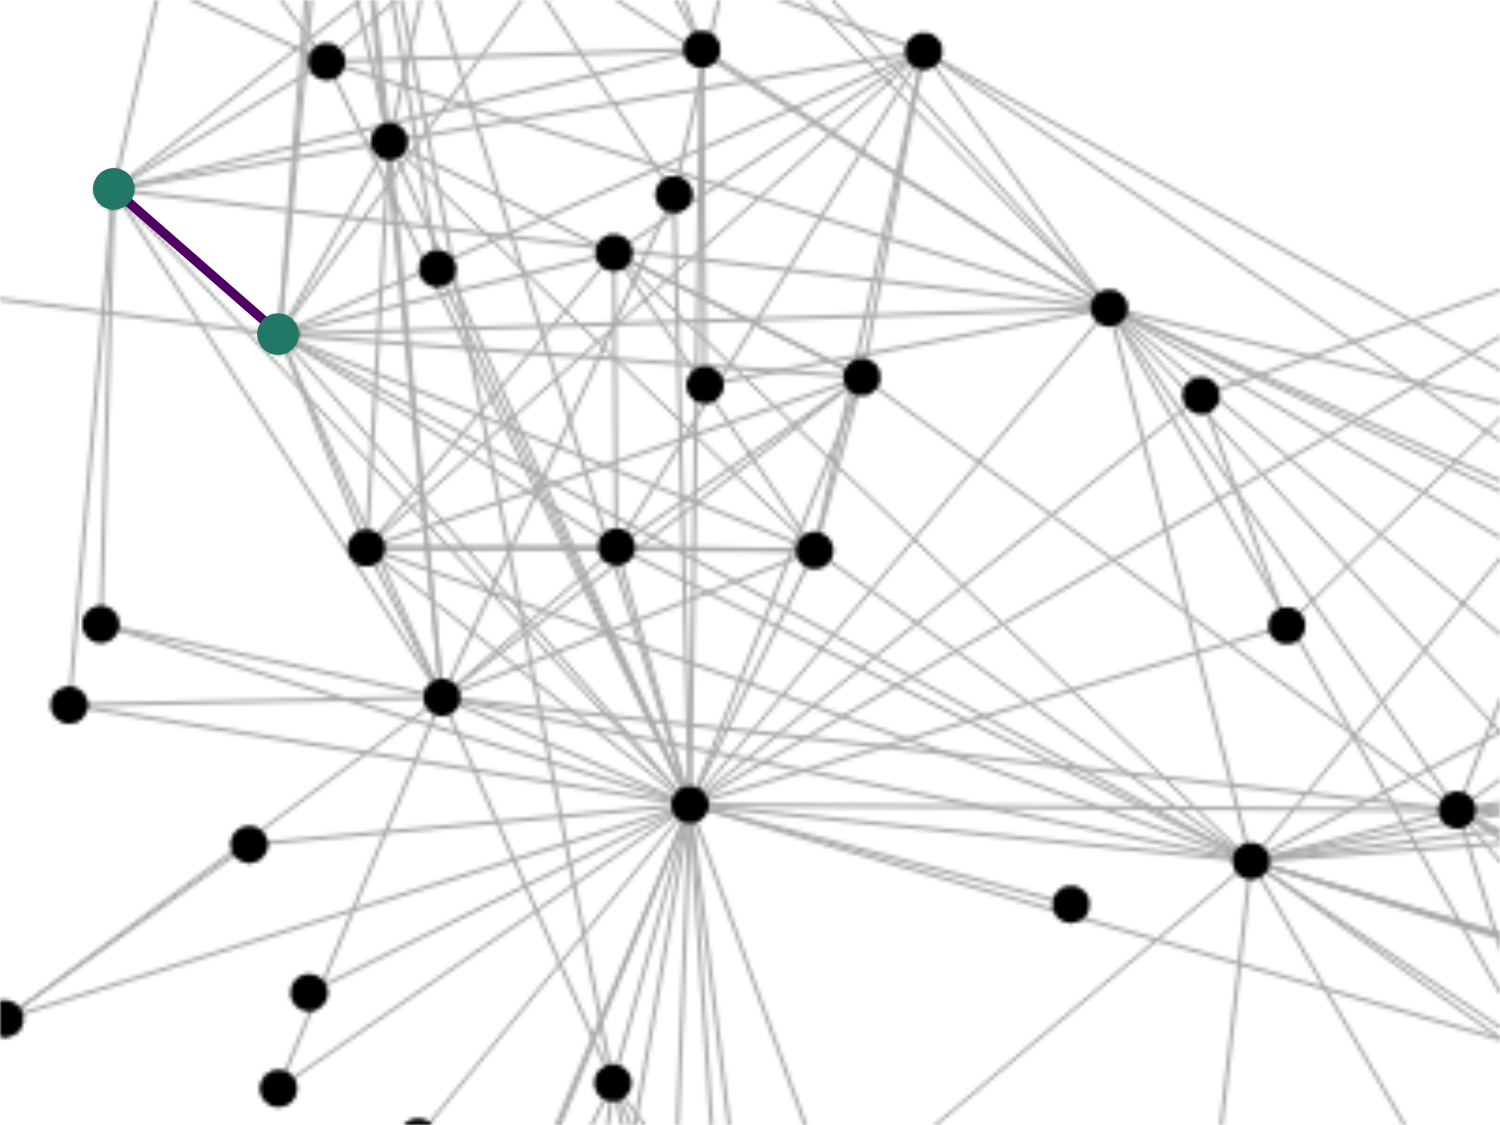
\includegraphics[width=5cm]{2a.png}
	
	\item[(b)]Zooming in, but keeping the same sizes for each node. Thereby the nodes will split up eventually. This process can be seen in the picture below, where we zoomed into the upper left corner with a focus on the big node in the middle, which can be hardly seen in the original picture.
	This process might consume a lot of time, depending on how many markers must be selected, it can be possible that the user has to zoom in quite a bit for several times. 
	
	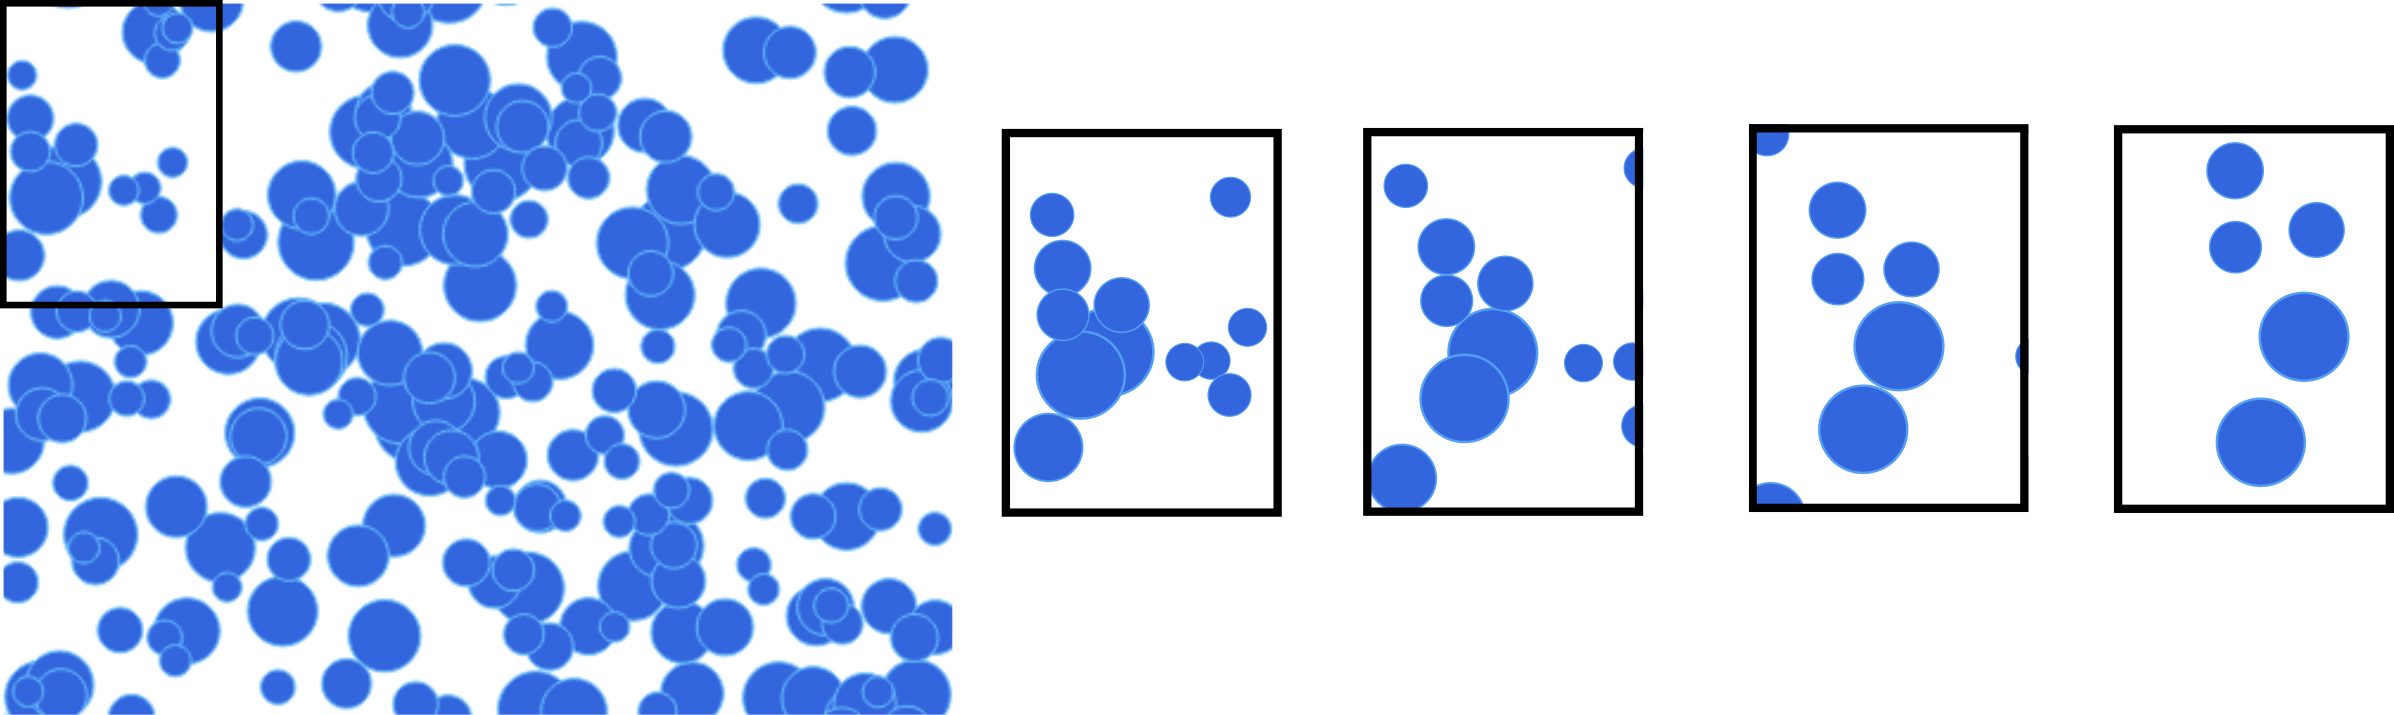
\includegraphics[width=\linewidth]{2b.png}
	
	\item[(c)]On the side there is a filter where you can select different colors. 
	The nodes of the selected color are getting bigger and thereby easier to select. 
	In the example below, the pink and light blue nodes are selected. 
	Obviously, there will be the same problem of overlapping markers, if all nodes are selected. 
	But this can be solved by just selecting the needed ones. 
	
	%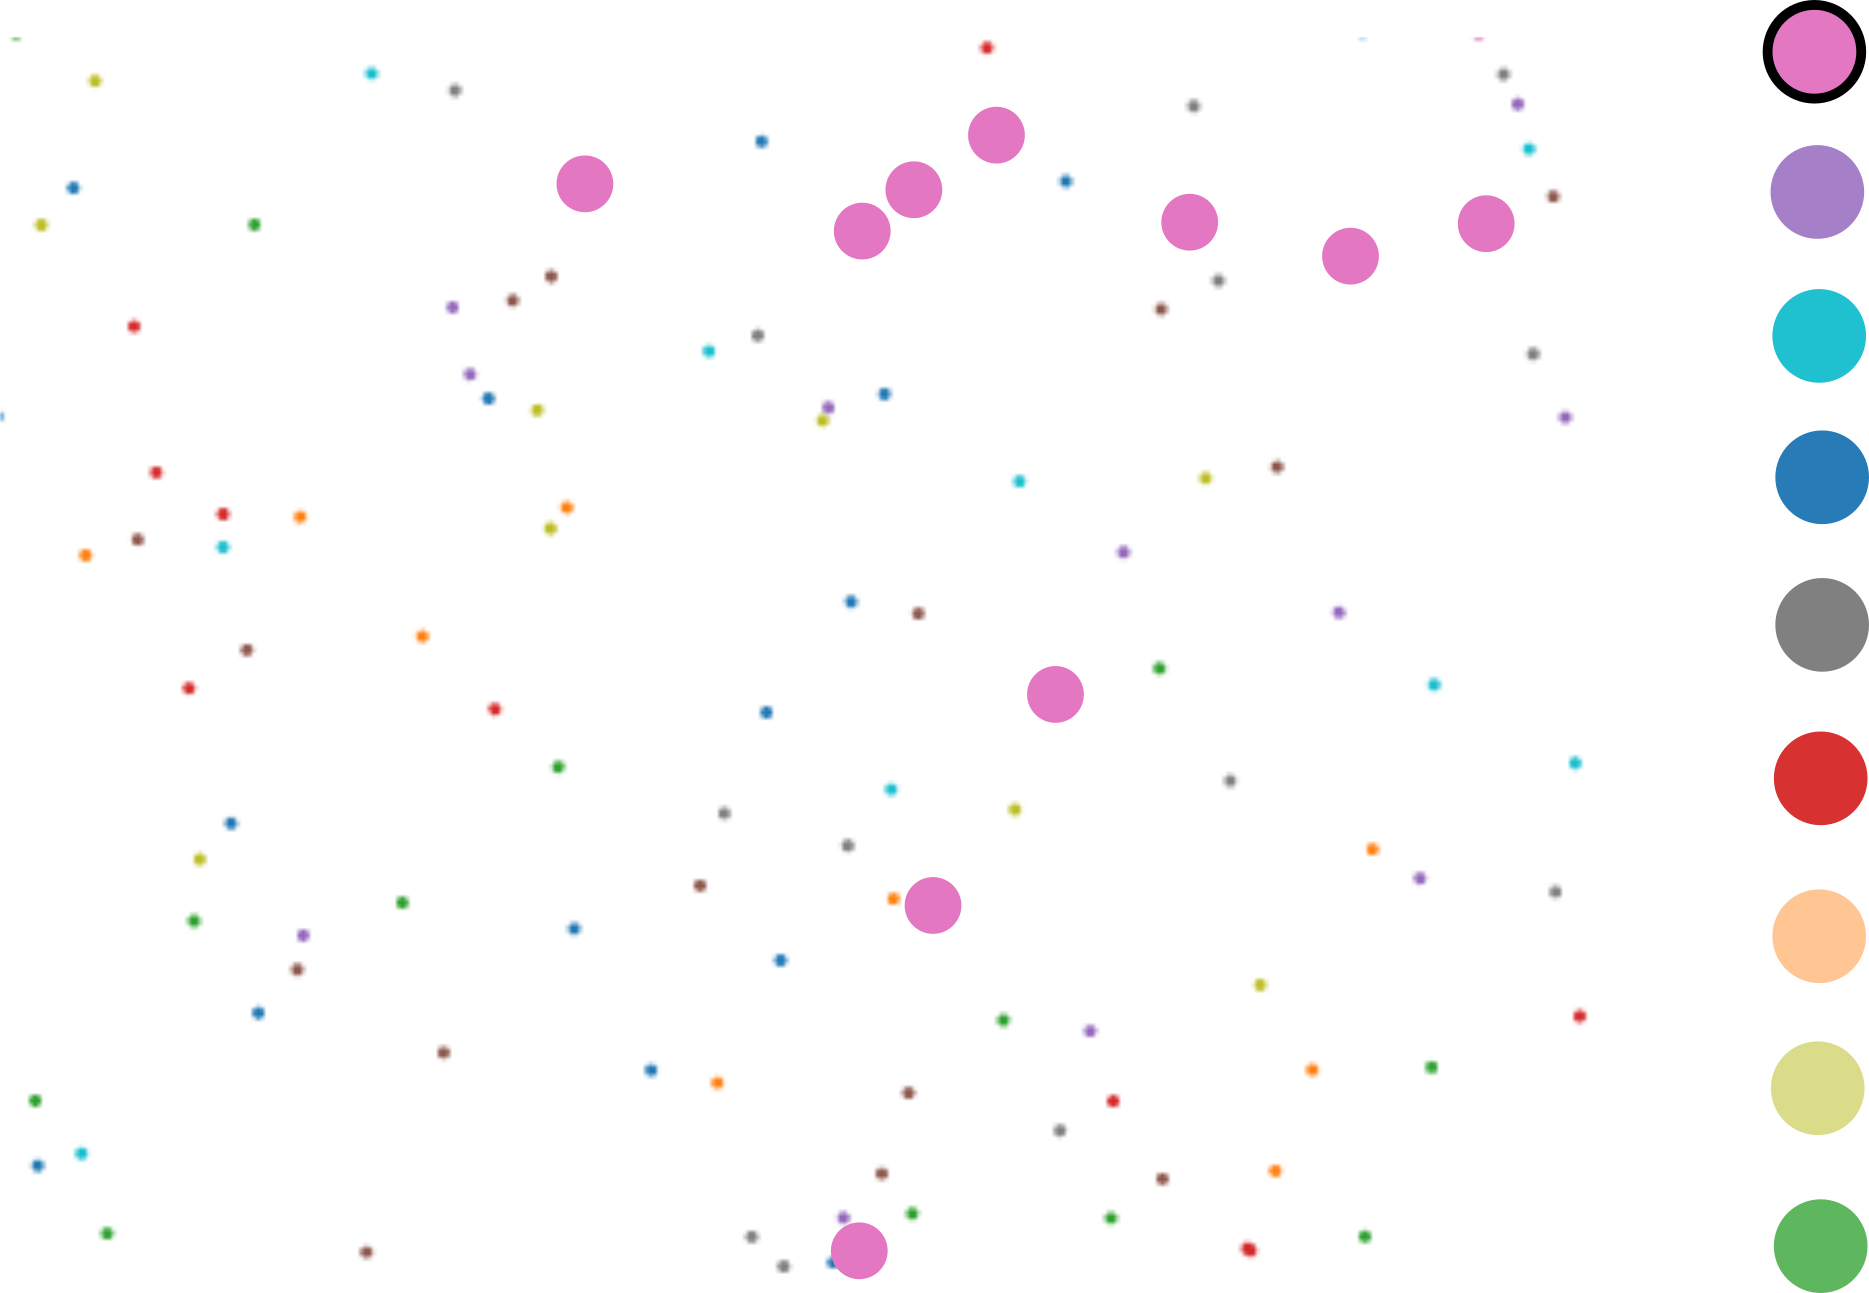
\includegraphics[width=\linewidth]{2c.png}
	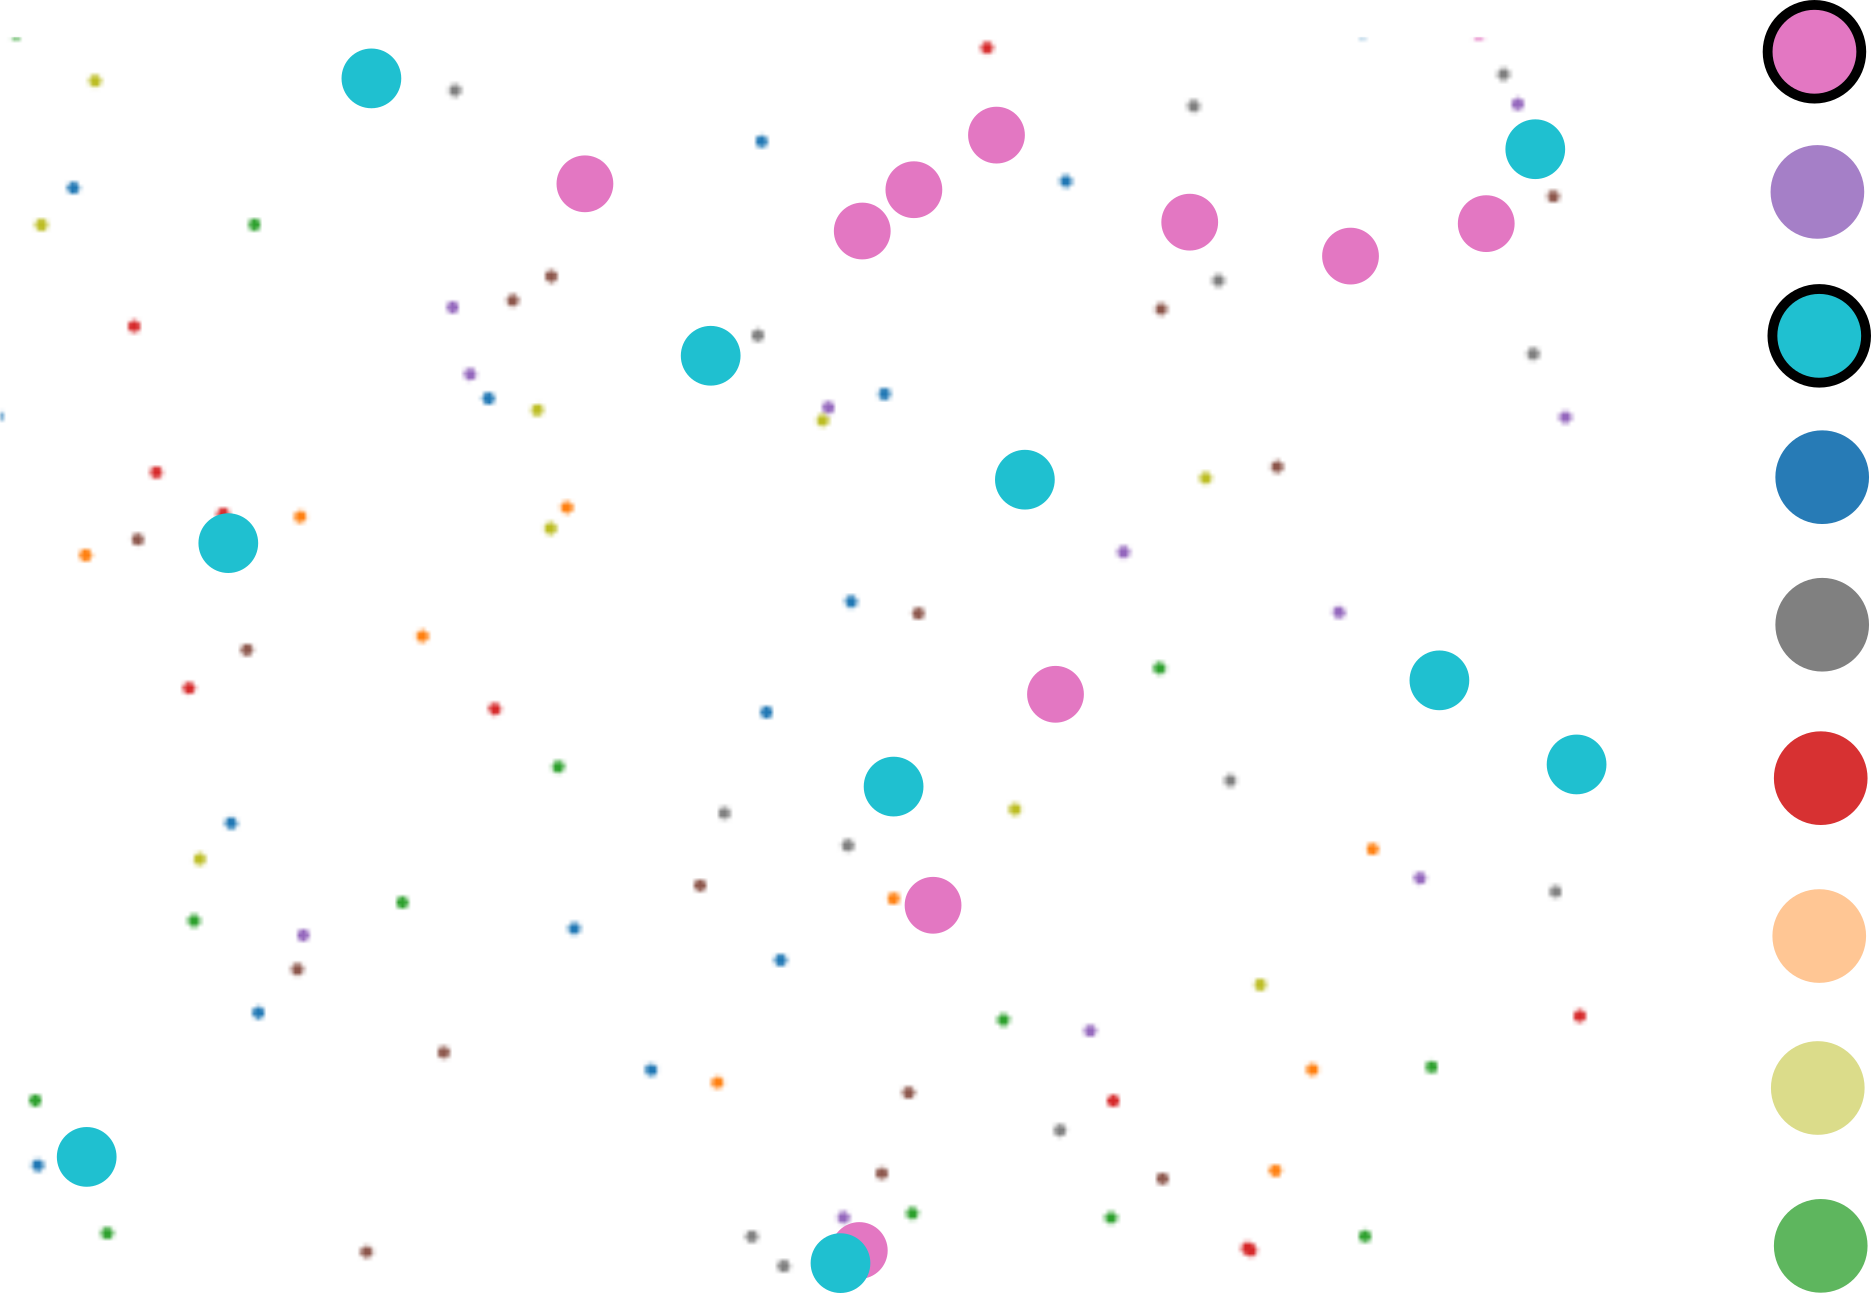
\includegraphics[height=5cm]{2c2.png}
\end{enumerate}

\clearpage
\section*{Task 3 - k-d Trees}
\begin{enumerate}
	\item[(a)] See \Cref*{1,2} for the resulting tree.
	
	\item[(b)] The problem with this tree is, that it is not balanced. 
	This can be fixed by taking the median point, that is changing the order of the given points in task (a). 
	The resulting tree can be seen in \Cref*{3,4}.
	
\end{enumerate}
\begin{figure}[!hb]
	\centering
	\begin{subfigure}[t]{.4\textwidth}
		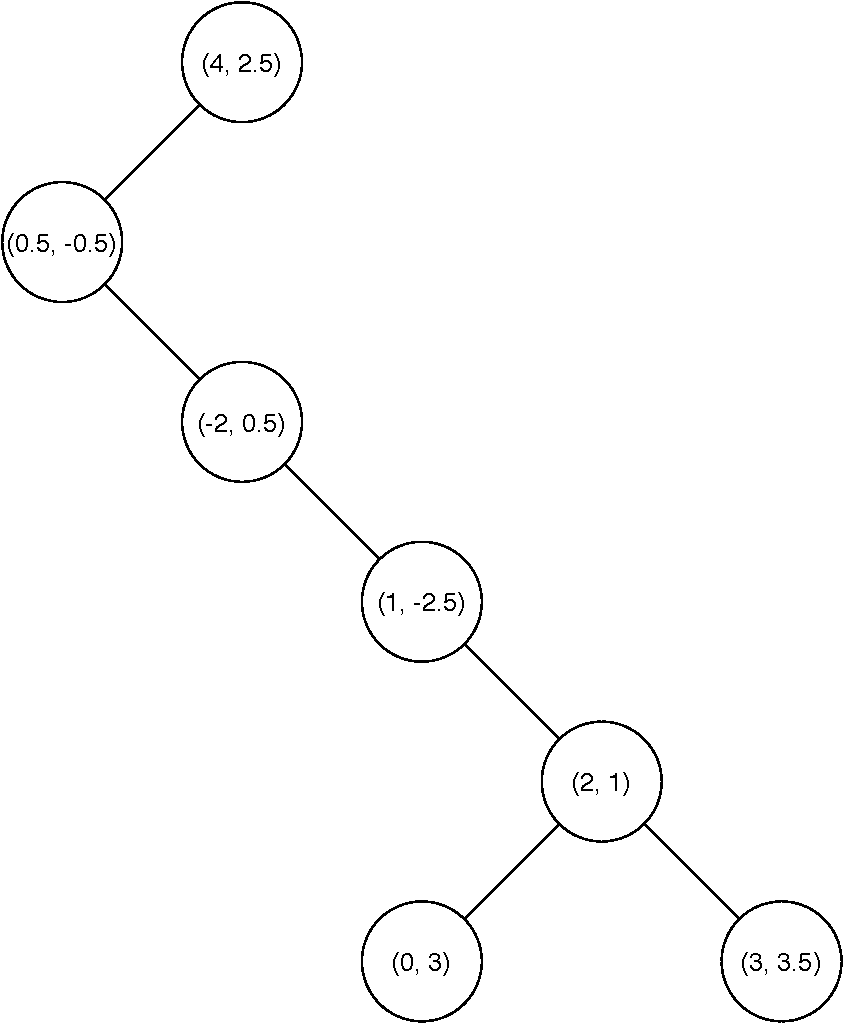
\includegraphics[height=5cm]{2-dtree.pdf}
		\caption{Data points visualised as areas.}
		\label{1}
	\end{subfigure}
	\begin{subfigure}[t]{.4\textwidth}
		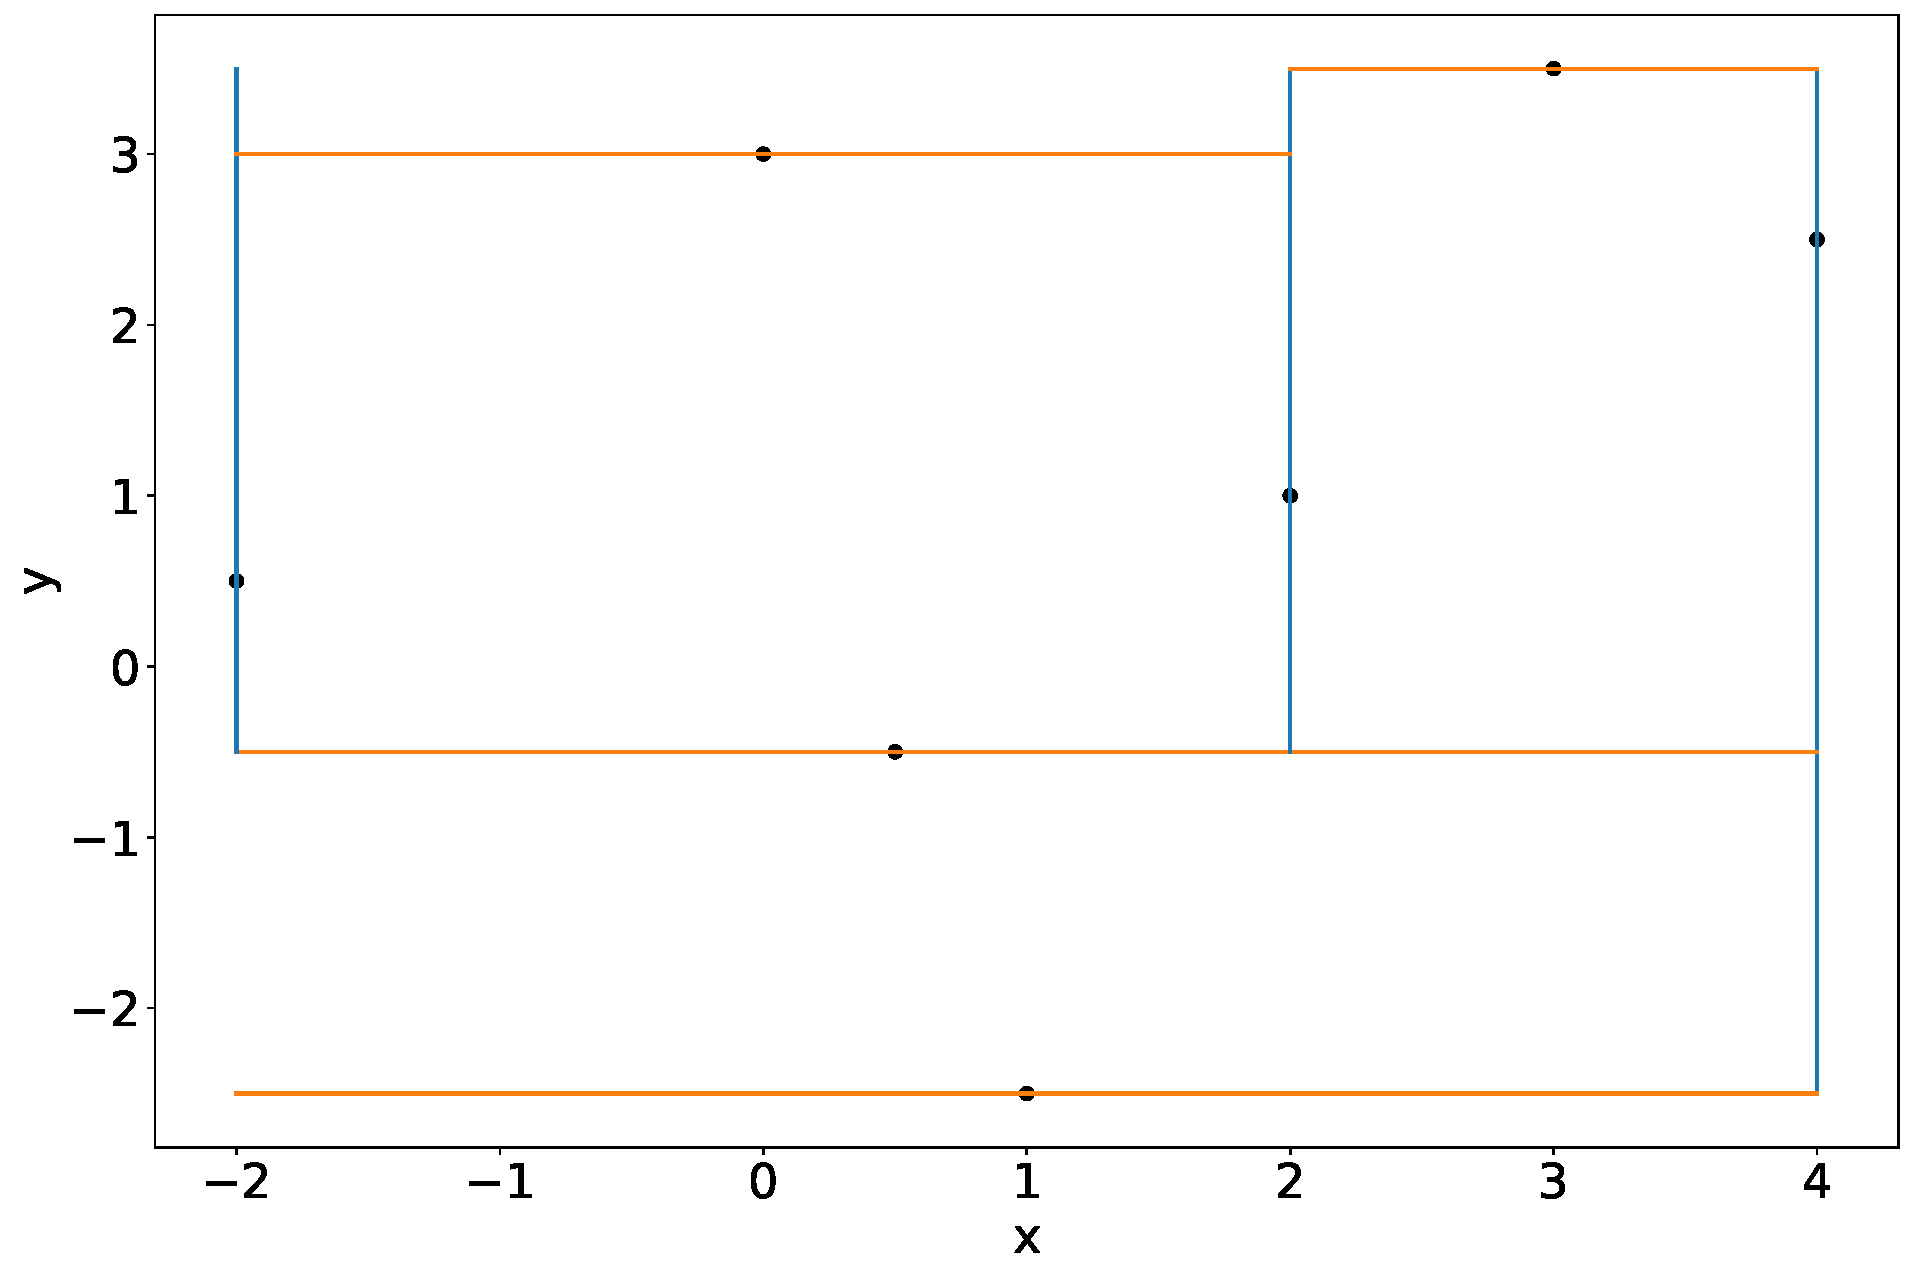
\includegraphics[width=\linewidth]{2dtree_nodelink.pdf}
		\caption{Data points visualised as a node-link diagram.}
		\label{2}
	\end{subfigure}
	\begin{subfigure}[t]{.4\textwidth}
		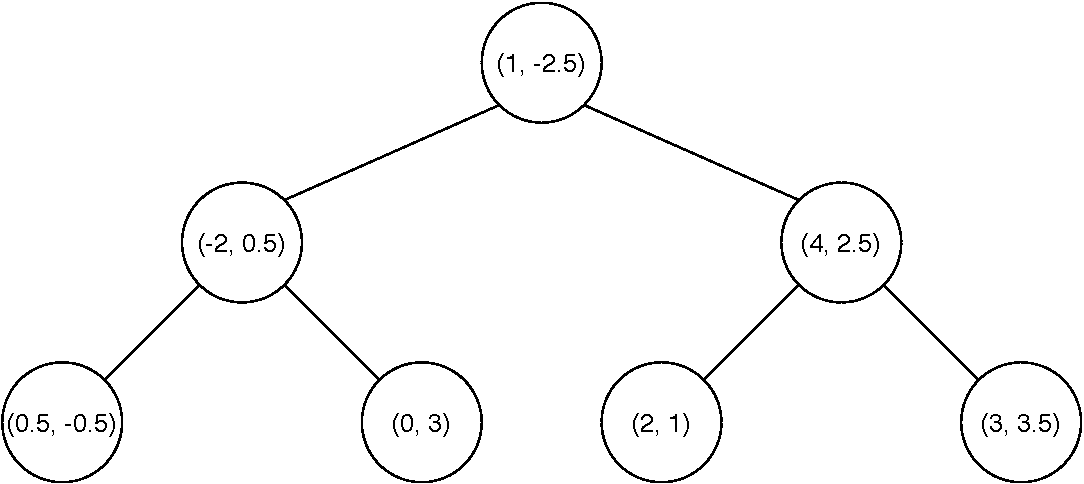
\includegraphics[width=\textwidth]{kd-tree2.pdf}
		\caption{Data points visualised as areas.}
		\label{3}
	\end{subfigure}
	\begin{subfigure}[t]{.4\textwidth}
		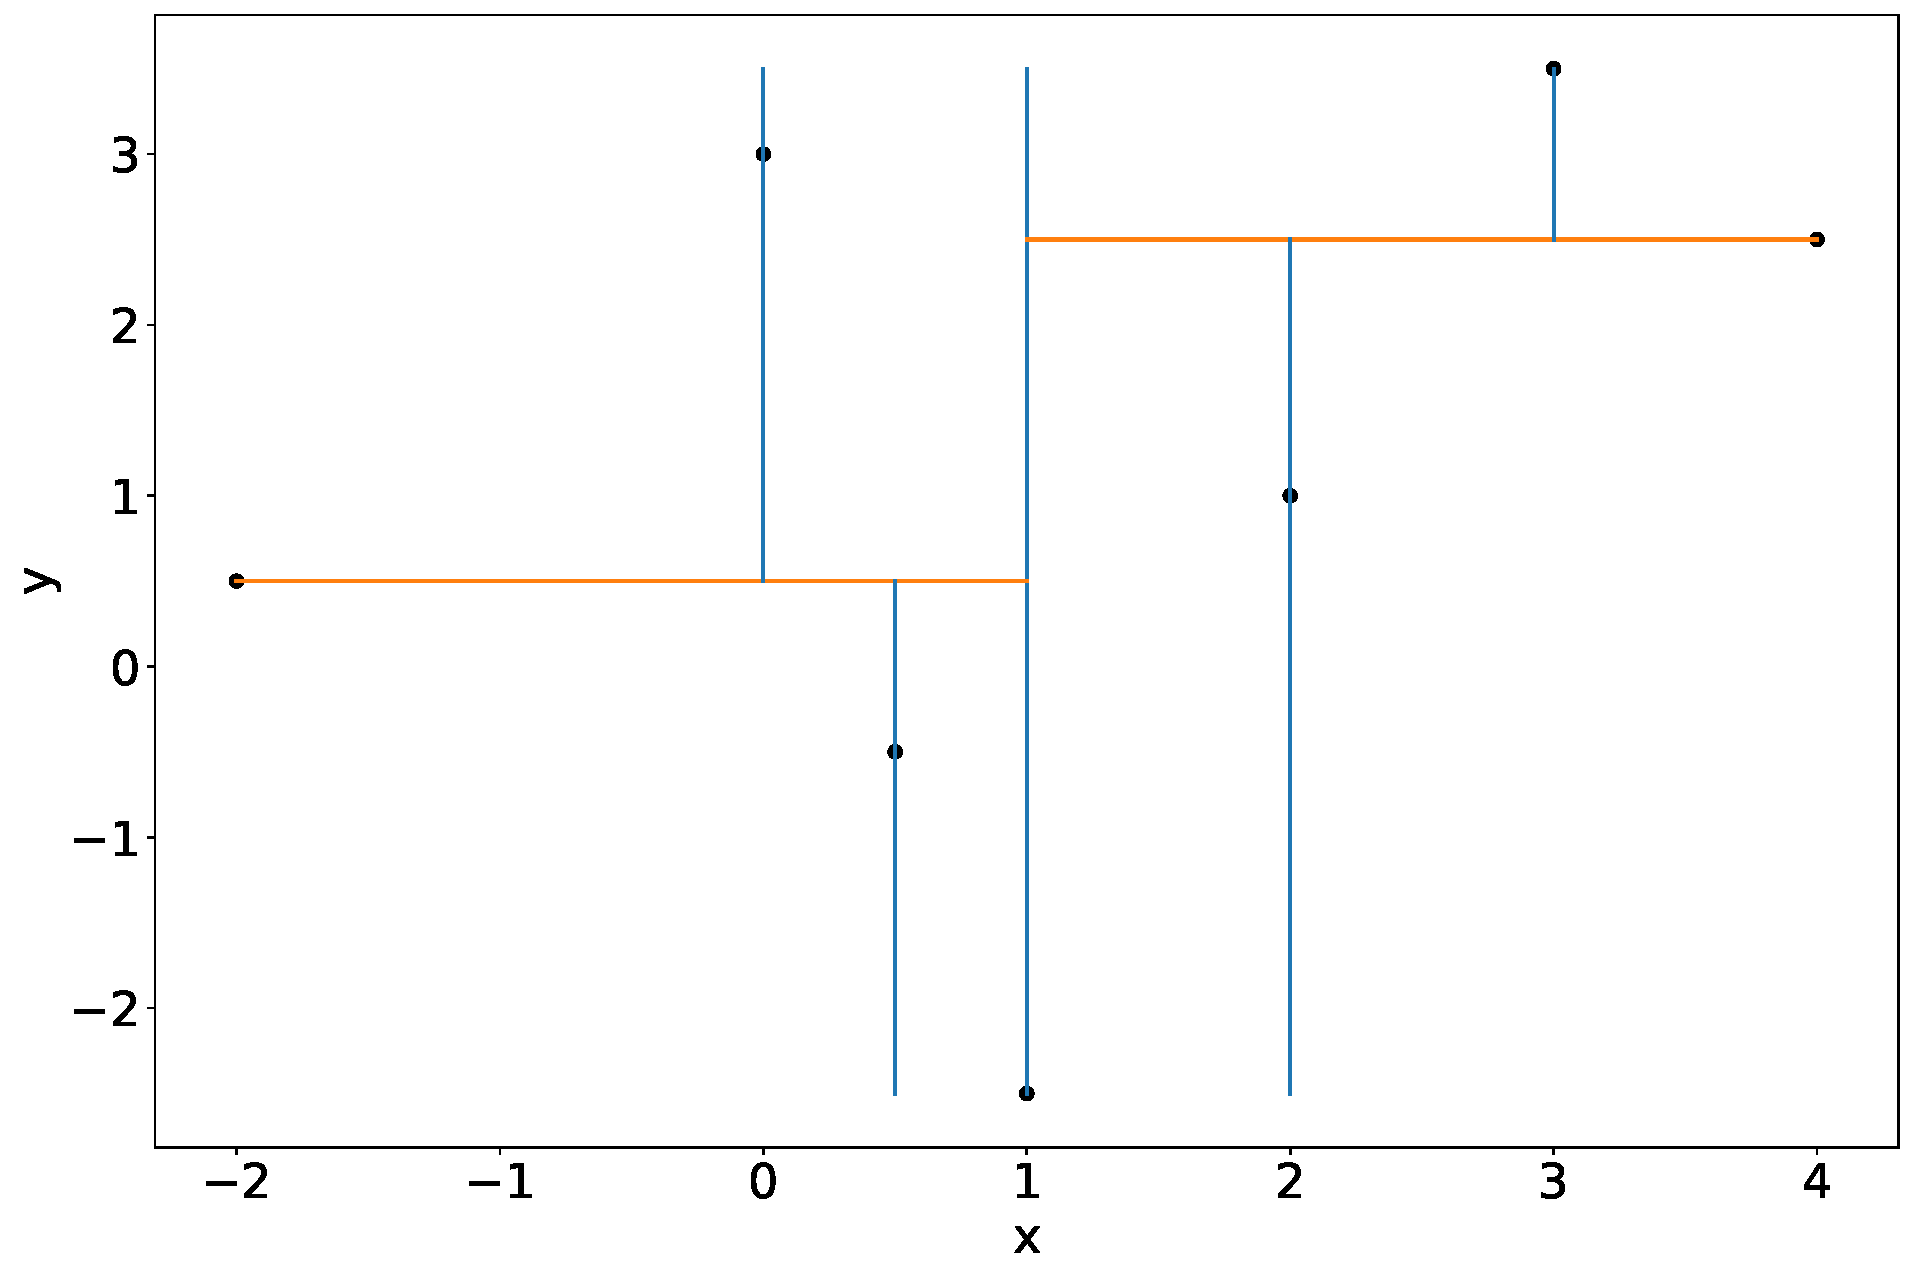
\includegraphics[width=\linewidth]{2dtree_nodelink2.pdf}
		\caption{Data points visualised as a node-link diagram.}
		\label{4}
	\end{subfigure}
	\caption{k-d Trees}
	\label{kdtree}
\end{figure}

\end{document}
